\chapter{St"orungstheorie\label{chapter:stoerungstheorie}}
\lhead{St"orungstheorie}
\rhead{}
Die St"orungstheorie geht davon aus, dass eine Basis von Zust"anden eines
quantenmechanischen Systems bereits bekannt ist. Eine kleine
"Anderung des Systems sollte sich dann in nur kleinen "Anderungen
der Zust"ande und ihrer Energieniveaus "aussern.
Diese Methode kann verwendet werden, um die Ver"anderung der Energieniveaus
eines Atoms zu berechnen, wenn dieses in ein "ausseres elektrisches Feld
oder ein "ausseres Magnetfeld gebracht wird.

\section{Grundprinzip der St"orungstheorie}
\rhead{Grundprinzip}
\index{stoerungstheorie@St\"orungstheorie!Prinzip}
Wir beginnen die Untersuchung mit einer Anwendung auf die Nullstellen
eines quadratischen Polynoms. Sei also
\[
p(x) = ax^2 + bx + c
\]
ein quadratisches Polynom, nat"urlich k"onnen wir sofort die Nullstellen
mit Hilfe der L"osungsformel
\begin{equation}
x_{\pm}=\frac{-b\pm\sqrt{b^2-4ac}}{2a}
\label{skript:mitternachtsformel}
\end{equation}
finden.  Ver"andert man die Koeffizienten von $p(x)$, werden sich auch
die beiden Nullstellen ver"andern, sie k"onnen mit der Formel
(\ref{skript:mitternachtsformel}) bestimmt werden.

Nehmen wir also an, dass die Koeffizienten $a$, $b$ und $c$ von $p(x)$
von einem Parameter $\varepsilon$ abh"angen. Statt der Konstanten verwenden
wir also Funktionen
\begin{align*}
a(\varepsilon)&=a_0+a_1\varepsilon+a_2\varepsilon^2+\dots\\
b(\varepsilon)&=b_0+b_1\varepsilon+b_2\varepsilon^2+\dots\\
c(\varepsilon)&=c_0+c_1\varepsilon+c_2\varepsilon^2+\dots
\end{align*}
von $\varepsilon$. Mit diesen Koeffizienten wird aus dem Polynom $p(x)$
eine Familie von Polynomen
\[
p_\varepsilon(x)=a(\varepsilon)x^2 + b(\varepsilon)x+c(\varepsilon).
\]
Die L"osungsformel (\ref{skript:mitternachtsformel}) liefert weiterhin die
Nullstellen von $p_{\varepsilon}(x)=0$.
Sei $x_0$ eine der Nullstellen von $p_0(x) = 0$.

Statt die L"osungen von $p_{\varepsilon}(x)=0$ mit Hilfe der L"osungsformel
zu finden, k"onnen wir auch versuchen, von $x_0$ ausgehend eine N"aherung
zu finden. Diese L"osung wird von $\varepsilon$ abh"angen, wir setzen
die Abh"angigkeit als Potenzreihe
\begin{equation}
x_\varepsilon = x_0 + x_1\varepsilon +x_2 \varepsilon^2+\dots
\label{skript:stoerungsansatz}
\end{equation}
an.
\begin{figure}
\centering
\includegraphics[width=0.55\hsize]{graphics/pert-1.pdf}
\caption{St"orungsl"osung f"ur die Abh"angigkeit der L"osung einer
quadratischen Gleichung $a(\varepsilon)x^2+b(\varepsilon)x+c(\varepsilon)=0$
in Abh"angigkeit von $\varepsilon$,
mit $a(\varepsilon)=1+\varepsilon$, $b(\varepsilon)=\varepsilon$ und
$c(\varepsilon)=-1+\varepsilon$. Exakte L"osung {\color{red} rot}, 
St"orungsapproximation erster Ordnung {\color{blue} blau}.
\label{skript:stoerungsloesung}}
\end{figure}
Wir nennen die Potenzreihe (\ref{skript:stoerungsansatz}) f"ur die L"osung
von $p_\varepsilon(x)=0$ die St"orungsreihe f"ur $x_\varepsilon$.
Setzen wir (\ref{skript:stoerungsansatz}) in die Gleichung $p_{\varepsilon}(x)=0$
ein, ergibt sich die Gleichung
\begin{align*}
0&=a(\varepsilon)x_\varepsilon^2+b(\varepsilon)x_\varepsilon+c(\varepsilon)
\\
&=
(a_0+a_1\varepsilon+a_2\varepsilon^2+\dots)
(x_0+x_1\varepsilon+x_2\varepsilon^2+\dots)^2\\
&\qquad
+
(b_0+b_1\varepsilon+b_2\varepsilon^2+\dots)
(x_0+x_1\varepsilon+x_2\varepsilon^2+\dots)\\
&\qquad
+
(c_0+c_1\varepsilon+c_2\varepsilon^2+\dots)
\\
&=
(a_0+a_1\varepsilon+a_2\varepsilon^2+\dots)
(x_0^2+2x_0x_1\varepsilon +x_1^2\varepsilon^2+2x_0x_2\varepsilon^2+\dots)
\\
&\qquad
+
b_0x_0 + (b_0x_1+b_1x_0)\varepsilon+(b_0x_2+b_1x_1+b_2x_0)\varepsilon+\dots\\
&\qquad
+
c_0+c_1\varepsilon+c_2\varepsilon^2+\dots
\\
&=
a_0x_0^2 + (2a_0x_0x_1 + a_1x_0^2)\varepsilon +
(a_2x_0^2 + 2a_1x_0x_1 + a_0x_1^2 +2a_0x_0x_2)\varepsilon^2+\dots
\\
&\qquad
+
b_0x_0 + (b_0x_1+b_1x_0)\varepsilon+(b_0x_2+b_1x_1+b_2x_0)\varepsilon^2+\dots\\
&\qquad
+
c_0+c_1\varepsilon+c_2\varepsilon^2+\dots
\\
&=
a_0x_0^2 + b_0x_0+c_0
+(2a_0x_0x_1+a_1x_0^2+b_0x_1+b_1x_0+c_1)\varepsilon
\\
&\qquad
+(
a_2x_0^2 + 2a_1x_0x_1 + a_0x_1^2 +2a_0x_0x_2
+b_0x_2+b_1x_1+b_2x_0
+c_2
)\varepsilon^2+\dots
\end{align*}
Der konstante Term in der letzten Form dieser Gleichung ist $p_0(x_0)$, 
da $x_0$ eine Nullstelle ist, muss er verschwinden. Wenn die Gleichung
f"ur alle $\varepsilon$ erf"ullt sein soll, dann muss auch der
Koeffizient von $\varepsilon$ verschwinden, es muss also gelten
\begin{align}
2a_0x_0x_1+a_1x_0^2+b_0x_1+b_1x_0+c_1&= 0
\label{skript:stoerung-1ordnung}
\\
(2a_0x_0+b_0)x_1&=-(a_1x_0^2+b_1x_0+c_1)\\
x_1&=-
\frac{a_1x_0^2+b_1x_0+c_1}{2a_0x_0+b_0}.
\notag
\end{align}
Damit ist eine erste Approximation von $x_\varepsilon$ gefunden:
\[
x_\varepsilon\simeq x_0 -
\frac{a_1x_0^2+b_1x_0+c_1}{2a_0x_0+b_0}\varepsilon.
\]
Man nennt dies die St"orungsapproximation erster Ordnung (in $\varepsilon$).

Man kann die Approximation noch verbessern, indem man auch noch den
Koeffizienten von $\varepsilon^2$ in $x_\varepsilon$ berechnet.
Dazu verwendet man, dass in der Gleichung auch der Koeffizient von
$\varepsilon^2$ verschwinden muss:
\begin{align*}
a_2x_0^2 + 2a_1x_0x_1 + a_0x_1^2 +2a_0x_0x_2
+b_0x_2+b_1x_1+b_2x_0
+c_2
&=0
\\
(2a_0x_0+b_0)x_2
+a_2x_0^2 + 2a_1x_0x_1 + a_0x_1^2
+b_1x_1+b_2x_0
+c_2&=0
\end{align*}
Daraus kann man schliessen, dass
\[
x_2=-\frac{
a_2x_0^2 + 2a_1x_0x_1 + a_0x_1^2
+b_1x_1+b_2x_0
+c_2
}{2a_0x_0+b_0}.
\]
Mit den Koeffizienten $x_1$ und $x_2$ erh"alt man die St"orungsapproximation
zweiter Ordnungn.

Die St"orungsapproximation scheint also zu funktionieren, solange
der Nenner $2a_0x_0+b_0$ gross ist. Dann werden n"amlich die 
Koeffizienten $x_1$ und $x_2$ klein sein. Problematisch wird
die Approximation in dem Falle, wo $2a_0x_0+b_0$ verschwindet.
Setzt man allerdings die L"osungsformel (\ref{skript:mitternachtsformel}) f"ur
$x_0$ ein, erh"alt man
\begin{align*}
2a_0x_0+b_0&=2a_0\frac{-b_0\pm\sqrt{b_0^2-4a_0c_0}}{2a_0}+b_0      \\
           &=\pm\sqrt{b_0^2-4a_0c_0}.
\end{align*}
Der Radikand ist die Diskriminante der unspr"unglichen quadratischen
Gleichung.
\begin{figure}
\centering
\includegraphics{graphics/pert-3.pdf}
\caption{Aufspaltung der doppelten Nullstelle $x_0=1$ von
$p_\varepsilon(x)=x^2-2x+1-\varepsilon$
\label{skript:entartetenullstellen}}
\end{figure}
Der Nenner verschwindet also genau dann, wenn die quadratische
Gleichung eine doppelte Nullstelle hat. In diesem Fall spaltet sich
die eine doppelte L"osung in zwei verschiedene L"osungen $x_{\pm}$ auf,
wie das in Abbildung~\ref{skript:entartetenullstellen} f"ur
das Polynom $p_{\varepsilon}=x^2-2x+1-\varepsilon$ dargestellt ist.
Es ist klar, dass es keine Funktion der Form
(\ref{skript:stoerungsansatz}) 
gibt, die diese Aufspaltung wiedergeben kann.


Wir fassen zusammen, was wir hier als L"osungsmethode gefunden haben:
\begin{enumerate}
\item Gegeben ist eine Gleichung $F_\varepsilon(x)=0$, gesucht
sind die L"osungen $x_\varepsilon$ der Gleichung in Abh"angigkeit von
$\varepsilon$.
\item Die L"osung $x_0$ der Gleichung f"ur den Parameterwert $\varepsilon=0$
ist bekannt.
\item Setze die L"osung in Form einer Potenzreihe an:
$x_\varepsilon = x_0+x_1\varepsilon+x_2\varepsilon^2+\dots$
\item Setze den L"osungsansatz in die Gleichung $F_\varepsilon(x)=0$ ein
und ermittle die Koeffizienten $x_1,x_2,\dots$ durch Koeffizientenvergleich.
\end{enumerate}
Schritt~4 ist eventuell nicht direkt durchf"uhrbar, wenn die Funktion
$F_\varepsilon(x)$ zu kompliziert ist. Man kann aber immer versuchen, die
Funktion als Potenzreihe in $x$ auszudr"ucken, 
\[
F_\varepsilon(x)=F_\varepsilon(x_0) + DF_\varepsilon(x_0)\cdot x
+ \frac12 D^2F_\varepsilon(x_0)\cdot(x,x)+\dots,
\]
und dann die Koeffizienten dieser Potenzreihe als Potenzreihe in $\varepsilon$.
So entsteht auf jeden Fall eine Vektorgleichung, deren Komponenten nur
Polynome in $\varepsilon$ sind, f"ur die sich Schritt~4 durchf"uhren l"asst.

\section{St"orungstheorie in der Quantenmechanik}
\rhead{St"orungstheorie in der Quantenmechanik}
Es sei $H_0$ der Hamilton-Operator eines quantenmechanischen Systems
mit den Eigenvektoren $|\psi_0^{(0)}\rangle$, $|\psi_1^{(0)}\rangle,\dots$
und Energien
$E_0^{(0)}$, $E_1^{(0)},\dots$.
Es gilt also 
\[
H_0\,|\psi_i^{(0)}\rangle = E_i^{(0)}\,|\psi_i^{(0)}\rangle.
\]
Der Hamilton-Operator $H_0$ wird nun durch einen zus"atzlichen Term
$H_1$ ver"andert. Wir gehen davon aus, dass $H_1$ im Vergleich zu
$H_0$ nur schwache Effekte beschreibt. Der neue Operator ist
\[
H(\varepsilon)=H_0+\varepsilon H_1.
\]
Darin ist $\varepsilon\ll 1$ ein kleiner Parameter, der ausdr"ucken
soll, dass $H_1$ den Operator nur ganz wenig "andert, insbesondere
sind die Zust"ande und Eigenwerte von $E(\varepsilon)$ nahe bei 
den $E_i^{(0)}$ und $\psi_i^{(0)}$.

Bringt man ein Atom in elektrisches oder magnetisches Feld, "andern
sich die Energieniveaus.
Die technische realisierbaren Felder sind typischerweise bedeutend
schw"acher als das Coulombpotential des Atomkernes.
Man kann solche Felder also als St"orungen des Hamiltonoperators
des Atoms betrachten.

Die Aufgabe der St"orungstheorie ist, die Zust"ande
$|\psi_i(\varepsilon)\rangle$
und Energien $E_i(\varepsilon)$ mit
\[
H(\varepsilon)\,|\psi_i(\varepsilon)\rangle
=
E_i(\varepsilon)\,|\psi_i(\varepsilon)\rangle
\]
mindestens n"aherungsweise zu bestimmen.
Wir versuchen $E_i(\varepsilon)$ und $|\psi_i(\varepsilon)\rangle$ als
Reihenentwicklung auszudr"ucken:
\begin{align*}
E_k(\varepsilon)
&=
E_k^{(0)}+\varepsilon E_k^{(1)} + \varepsilon^2 E_k^{(2)}+\dots
\\
|\psi_k(\varepsilon)\rangle
&=
|\psi_k^{(0)}\rangle+\varepsilon\,|\psi_k^{(1)}\rangle
+\varepsilon^2\,|\psi_k^{(2)}\rangle+\dots
\end{align*}
Das gestellte Problem ist in erster N"aherung gel"ost, wenn wir $E_k^{(1)}$
und $\psi_k^{(1)}$ bestimmt haben.

%Die Eigenvektoren $\psi_k^{(0)}$ bilden eine Basis des Hilbertraumes,
%also m"ussen sich auch die modifizierten Eigenvektoren in dieser Basis
%ausdr"ucken lassen:
%\[
%|\psi_k(\varepsilon)\rangle=|\psi_k\rangle +\sum_{l=0}^\infty a_{kl}(\varepsilon)|\psi_l\rangle,
%\]
%wobei die Koeffizienten $a_{kl}(\varepsilon)$ klein sind.
%Das Problem ist gel"ost, wenn die $a_{kl}(\varepsilon)$ bestimmt sind.

\section{Erste N"aherung\label{section:erstenaeherung}}
\rhead{Erste N"aherung}
Wir wenden jetzt den Operator $H_0+\varepsilon H_1$ auf
$|\psi_k(\varepsilon)\rangle$ an, und behalten die Terme erster Ordnung
\begin{align*}
(H_0+\varepsilon H_1)\,|\psi_k(\varepsilon)\rangle
&=
E_k(\varepsilon)\,|\psi_k(\varepsilon)\rangle
\\
H_0\,|\psi_k^{(0)}\rangle +\varepsilon H_1\,|\psi_k^{(0)}\rangle
+\varepsilon H_0\,|\psi_k^{(1)}\rangle
+\dots
&=
E_k^{(0)}\,|\psi_k^{0}\rangle + \varepsilon E_k^{(1)} \,|\psi_k^{(0)}\rangle
+ \varepsilon E_k^{(0)} \,|\psi_k^{(1)}\rangle + \dots
\end{align*}
Die jeweils ersten Terme sind gleich, da ja $|\psi_k^{(0)}\rangle$
Eigenvektoren von $H_0$ sind mit Eigenwert $E_k^{(0)}$. Wir subtrahieren sie,
und k"onnen dann durch $\varepsilon$ teilen:
\begin{align*}
H_1\,|\psi_k^{(0)}\rangle
+H_0\,|\psi_k^{(1)}\rangle
+ \dots
&=
E_k^{(1)}\,|\psi_k^{(0)}\rangle + E_k^{(0)} \,|\psi_k^{(1)}\rangle+\dots
\end{align*}
Die Punkte stehen f"ur Terme, die minstens einen Faktor $\varepsilon$
enthalten.
Aus diesen Gleichungen m"ussen wir $E_k^{(1)}$ und $|\psi_k^{(1)}\rangle$
bestimmen. Dazu multiplizieren wir $\langle \psi_l^{(0)}|$.
Da die ungest"orten Eigenfunktionen orthogonal sind, kann der erste
Term auf der rechten Seite durch $\delta_{kl}E_k^{(0)}$ ersetzt werden,
man bekommt
\begin{equation}
\begin{aligned}
\langle \psi_l^{(0)}|\, H_1 \,|\psi_k^{(0)}\rangle
+
\langle \psi_l^{(0)}|\, H_0 \,|\psi_k^{(1)}\rangle
&=
E_k^{(1)}\langle\psi_l^{(0)}|\psi_k^{(0)}\rangle
+
E_k^{(0)}\langle\psi_l^{(0)}|\psi_k^{(1)}\rangle
\\
&=
\delta_{kl} E_k^{(1)}
+
E_k^{(0)}\langle\psi_l^{(0)}|\psi_k^{(1)}\rangle.
\end{aligned}
\label{skript:pert-1}
\end{equation}
Da $H_0$ selbstadjungiert ist, kann man auch den zweiten Term auf der
linken Seite aufl"osen:
\[
\langle\psi_l^{(0)}|\,H_0\,|\psi_k^{(1)}\rangle
=
(\langle\psi_l^{(0)}|\,H_0)\,|\psi_k^{(1)}\rangle
=
\langle\psi_l^{(0)}|\,E_l^{(0)}\,|\psi_k^{(1)}\rangle
=
E_l^{(0)}\langle \psi_l^{(0)}|\psi_k^{(1)}\rangle.
\]
Die Gleichung (\ref{skript:pert-1}) wird damit zu
\begin{align*}
\langle \psi_l^{(0)}|\, H_1 \,|\psi_k^{(0)}\rangle
+
E_l^{(0)}\langle \psi_l^{(0)}|\psi_k^{(1)}\rangle
&=
\delta_{kl} E_k^{(1)}
+
E_k^{(0)}\langle\psi_l^{(0)}|\psi_k^{(1)}\rangle.
\end{align*}
Bringen wir den zweiten Term links auf die rechte Seite, erhalten wir
die Gleichung
\begin{align*}
\langle \psi_l^{(0)}|\, H_1 \,|\psi_k^{(0)}\rangle
&=
\delta_{kl} E_k^{(1)}
+
(E_k^{(0)}-E_l^{(0)})\langle\psi_l^{(0)}|\psi_k^{(1)}\rangle.
\end{align*}
Sie entspricht der Gleichung~(\ref{skript:stoerung-1ordnung})
des Einf"uhrungsbeispiels und erlaubt uns, die Koeffizienten
erster Ordnung der St"orungsreihe zu berechnen.

\section{Nicht entartete Zust"ande\label{section:nichtentartetezustaende}}
\rhead{Nicht entartete Zust"ande}
Falls die Zust"ande nicht entartet sind, sind alle Energiewerte
verschieden, und $E_k^{(0)}-E_l^{(0)}\ne 0$ f"ur $k\ne l$. 
Dann kann man die L"osung ablesen:
\begin{equation}
\begin{aligned}
k&=l
&&\Rightarrow&
E_k^{(1)}
&=
\langle \psi_k^{(0)}|\, H_1 \,|\psi_k^{(0)}\rangle
\\
k&\ne l
&&\Rightarrow&
\langle\psi_l^{(0)}|\psi_k^{(1)}\rangle
&=
\frac{\langle \psi_l^{(0)}|\, H_1 \,|\psi_k^{(0)}\rangle}{E_k^{(0)}-E_l^{(0)}}
\end{aligned}
\label{skript:stoerungsloesung1ordnung}
\end{equation}
Durch diese Gleichungen ist nur der Koeffizient
$\langle\psi_k^{(0)}|\psi_k^{(1)}\rangle$
noch nicht bestimmt.

Mit den Koeffizienten $\langle\psi_l^{(0)}|\psi_k^{(0)}\rangle$ kann
man jetzt den neuen Zustand in erster N"aherung ausdr"ucken:
\begin{equation}
|\psi_k(\varepsilon)\rangle
=
|\psi_k^{(0)}\rangle
\langle\psi_k^{(0)}|\psi_k^{(1)}\rangle
+\varepsilon
\sum_{k\ne l}
\frac{\langle \psi_l^{(0)}|\, H_1 \,|\psi_k^{(0)}\rangle}{E_k^{(0)}-E_l^{(0)}}
\,
|\psi_l^{(0)}\rangle
\end{equation}
Darin ist nur der Koeffizient von $|\psi_k^{(0)}\rangle$ im ersten
Term auf der rechten Seite noch zu bestimmen.

Der fehlende Koeffizient muss so gew"ahlt werden, dass der neue
Vektor L"ange $1$ erh"alt.
Um $|\psi_k(\varepsilon)\rangle$ zu normieren, berechnen wir seine L"ange:
\begin{align}
1
&=
\langle\psi_k(\varepsilon)|\psi_k(\varepsilon)\rangle
\notag
\\
1
&=
\langle \psi_k^{(0)}|\psi_k^{(0)}\rangle
+
\varepsilon(
\langle \psi_k^{(1)}|\psi_k^{(0)}\rangle
+
\langle \psi_k^{(0)}|\psi_k^{(1)}\rangle
)
+
\varepsilon^2(
\langle \psi_k^{(2)}|\psi_k^{(0)}\rangle
+
\langle \psi_k^{(1)}|\psi_k^{(1)}\rangle
+
\langle \psi_k^{(0)}|\psi_k^{(2)}\rangle
)
+\dots
\label{skript:stoerungstheorie:norm}
\end{align}
Koeffizientenvergleich in~(\ref{skript:stoerungstheorie:norm}) liefert
\begin{align*}
0
&=
\langle \psi_k^{(1)}|\psi_k^{(0)}\rangle
+
\langle \psi_k^{(0)}|\psi_k^{(1)}\rangle
=
2\operatorname{Re}\langle \psi_k^{(1)}|\psi_k^{(0)}\rangle
\end{align*}
Daraus lesen wir ab, dass $\langle\psi_k^{(0)}|\psi_k^{(1)}\rangle$
rein imagin"ar sein, muss wir schreiben
\[
\langle\psi_k^{(0)}|\psi_k^{(1)}\rangle = i\gamma.
\]
Die Zahl $\gamma$ ist so zu w"ahlen, dass der neue Zustandsvektor
in erster N"aherung
\begin{equation}
|\psi_k(\varepsilon)\rangle
=
(1+i\varepsilon \gamma)
\,|\psi_k^{(0)}\rangle
+
\varepsilon
\sum_{k\ne l}
\frac{\langle \psi_l^{(0)}|\, H_1 \,|\psi_k^{(0)}\rangle}{E_k^{(0)}-E_l^{(0)}}
\,
|\psi_l^{(0)}\rangle
\end{equation}
normiert ist.

\section{Zweite N"aherung}
\rhead{Zweite N"aherung}
In den Abschnitten~\ref{section:erstenaeherung} und
\ref{section:nichtentartetezustaende} haben wir die Approximationsreihen
f"ur $E_k(\varepsilon)$ und $|\psi_k(\varepsilon)\rangle$
bis zu den linearen Termen entwickelt.
Mit etwas Aufwand k"onnen wir auch eine Approximation zweiter Ordnung
finden.
Dazu wenden wir wieder den Operator $H_0+\varepsilon H_1$
auf die Entwicklung $|\psi_k(\varepsilon)\rangle$, rechnen die Reihe aber bis
zu den Termen zweiter Ordnung aus
\begin{align*}
H_0\,|\psi_k^{(0)}\rangle
&+
\varepsilon
\bigl(
H_1\,|\psi_k^{(0)}\rangle
+
H_0\,|\psi_k^{(1)}\rangle
\bigr)
+
\varepsilon^2
\bigl(
H_0\,|\psi_k^{(2)}\rangle
+
H_1\,|\psi_k^{(1)}\rangle
\bigr)
+
\dots
\\
&=
E_k^{(0)}
+
\varepsilon
\bigl(
E_k^{(1)}\,|\psi_k^{(0)}\rangle
+
E_k^{(0)}\,|\psi_k^{(1)}\rangle
\bigr)
+
\varepsilon^2
\bigl(
E_k^{(2)}\,|\psi_k^{(0)}\rangle
+
E_k^{(1)}\,|\psi_k^{(1)}\rangle
+
E_k^{(0)}\,|\psi_k^{(2)}\rangle
\bigr)
+
\dots
\end{align*}
F"ur die Terme erster Ordnung haben wir den Koeffizientenvergleich
fr"uher schon durchgef"uhrt, hier vergleichen wir nur noch die
Koeffizienten der quadratischen Terme.
\begin{align*}
H_0\,|\psi_k^{(2)}\rangle
+
H_1\,|\psi_k^{(1)}\rangle
&=
E_k^{(2)}\,|\psi_k^{(0)}\rangle
+
E_k^{(1)}\,|\psi_k^{(1)}\rangle
+
E_k^{(0)}\,|\psi_k^{(2)}\rangle
\end{align*}
Auch hier brauchen wir wieder eine Entwicklung nach der Basis
$|\psi_l^{(0)}\rangle$, und multiplizieren deshalb mit
$\langle\psi_l^{(0)}|$:
\begin{align}
\langle\psi_l^{(0)}|\,H_0\,|\psi_k^{(2)}\rangle
+
\langle\psi_l^{(0)}|\,H_1\,|\psi_k^{(1)}\rangle
&=
E_k^{(2)}\langle\psi_l^{(0)}|\psi_k^{(0)}\rangle
+
E_k^{(1)}\langle\psi_l^{(0)}|\psi_k^{(1)}\rangle
+
E_k^{(0)}\langle\psi_l^{(0)}|\psi_k^{(2)}\rangle
\notag
\\
E_l^{(0)}\langle\psi_l^{(0)}|\psi_k^{(2)}\rangle
+
\langle\psi_l^{(0)}|\,H_1\,|\psi_k^{(1)}\rangle
&=
E_k^{(2)}\delta_{kl}
+
E_k^{(1)}\langle\psi_l^{(0)}|\psi_k^{(1)}\rangle
+
E_k^{(0)}\langle\psi_l^{(0)}|\psi_k^{(2)}\rangle
\notag
\\
(E_l^{(0)}-E_k^{(0)})\langle\psi_l^{(0)}|\psi_k^{(2)}\rangle
+
\langle\psi_l^{(0)}|\,H_1\,|\psi_k^{(1)}\rangle
&=
E_k^{(2)}\delta_{kl}
+
E_k^{(1)}\langle\psi_l^{(0)}|\psi_k^{(1)}\rangle
\label{skript:zweitenaeherung}
\end{align}
F"ur $k=l$ ist $E_l^{(0)}-E_k^{(0)}=0$ und die Gleichung kann nach 
$E_k^{(2)}$ aufgel"ost werden:
\begin{align*}
E_k^{(2)}
&=
\langle\psi_k^{(0)}|\, H_1\, |\psi_k^{(1)}\rangle
-E_k^{(1)}\langle\psi_k^{(0)}|\psi_k^{(1)}\rangle
\\
&=
\langle\psi_k^{(0)}|\, H_1\, |\psi_k^{(1)}\rangle
-i\gamma
\langle \psi_k^{(0)}|\, H_1 \,|\psi_k^{(0)}\rangle
\end{align*}
Den Vektor $|\psi_k^{(1)}\rangle$ kann man durch die im
Abschnitt~\ref{section:nichtentartetezustaende} gefundene
Entwicklung ersetzen, und erh"alt
\begin{align*}
E_k^{(2)}
&=
\langle\psi_k^{(0)}|\, H_1\,
\biggl(
i\gamma
\,|\psi_k^{(0)}\rangle
+
\sum_{k\ne l}
\frac{\langle \psi_l^{(0)}|\, H_1 \,|\psi_k^{(0)}\rangle}{E_k^{(0)}-E_l^{(0)}}
\,
|\psi_l^{(0)}\rangle
\biggr)
-i\gamma
\langle \psi_k^{(0)}|\, H_1 \,|\psi_k^{(0)}\rangle
\\
&=
i\gamma\langle\psi_k^{(0)}|\, H_1\, |\psi_k^{(0)}\rangle
+
\sum_{k\ne l}
\frac{\langle \psi_l^{(0)}|\, H_1 \,|\psi_k^{(0)}\rangle}{E_k^{(0)}-E_l^{(0)}}
\langle\psi_k^{(0)}|\, H_1 \,|\psi_l^{(0)}\rangle
-i\gamma
\langle \psi_k^{(0)}|\, H_1 \,|\psi_k^{(0)}\rangle
\\
&=
\sum_{k\ne l}
\frac{|\langle \psi_l^{(0)}|\, H_1 \,|\psi_k^{(0)}\rangle|^2}{E_k^{(0)}-E_l^{(0)}}.
\end{align*}
F"ur $k\ne l$ kann man $\langle\psi_l^{(0)}|\psi_k^{(2)}\rangle$ 
berechnen:
\begin{align*}
\langle\psi_l^{(0)}|\psi_k^{(2)}\rangle
&=
\frac1{E_l^{(0)}-E_k^{(0)}}\biggl(
E_k^{(1)}\langle\psi_l^{(0)}|\psi_k^{(1)}\rangle
-
\langle\psi_l^{(0)}|\,H_1\,|\psi_k^{(1)}\rangle
\biggr)
\\
&=
\frac{
\langle \psi_l^{(0)}|\, H_1 \,|\psi_k^{(0)}\rangle
\langle \psi_k^{(0)}|\, H_1 \,|\psi_k^{(0)}\rangle
}{
(E_k^{(0)}-E_l^{(0)})^2
}
+
\sum_{m\ne k}
\frac{\langle \psi_m^{(0)}|\, H_1 \,|\psi_k^{(0)}\rangle
\langle\psi_l^{(0)}|\, H_1 \,|\psi_m^{(0)}\rangle
}{
(E_k^{(0)}-E_m^{(0)})
(E_k^{(0)}-E_l^{(0)})
}
\end{align*}
Damit kann man jetzt auch die N"aherung zweiter Ordnung
f"ur die Zustandsvektoren $|\psi(\varepsilon)\rangle$
berechnen.
Wir verzichten darauf, die Formeln explizit darzustellen.

\section{Entartung}
\rhead{Entartung}
Da bei Entartung einge der Nenner in (\ref{skript:stoerungsloesung1ordnung})
verschwinden, kann die St"orungstheorie auf entartete Zust"ande
in dieser Form nicht angwendet werden.
Die Nenner w"aren kein Problem, wenn in (\ref{skript:stoerungsloesung1ordnung})
immer dann, wenn ein Nenner verschwindet, auch der zugeh"orige Z"ahler
verschwindet.
Wenn $|\psi_k^{(0)}\rangle$ und $|\psi_l^{(0)}\rangle$ den gleichen
Eigenwert im ungest"orten System haben, dann hat auch jede beliebige
Linearkombination den gleichen Eigenwert.
Das Problem ist also vor allem, dass wir im Eigenraum zu diesem
Eigenwert bisher eine unzweckm"assige Basis gew"ahlt haben.

Wir illustrieren diese an einem Beispiel in zwei Dimensionen:
\begin{beispiel}
Der Operator
\[
H_0=\begin{pmatrix}1&0\\0&1\end{pmatrix}
\]
hat in den Standardbasisvektoren zwei entartete Zust"ande, beide mit
Eigenwert $1$.
Wir st"oren diesen Operator mit 
\[
H_1=\begin{pmatrix} 0&1\\ 1&0 \end{pmatrix}.
\]
Dieses Problem k"onnen wir exakt l"osen, die charakteristische Gleichung
ist
\[
0=
\left|\begin{matrix}
1-\lambda&\varepsilon\\
\varepsilon&1-\lambda
\end{matrix}\right|
=(1-\lambda)^2-\varepsilon^2=(1-\lambda+\varepsilon)(1-\lambda-\varepsilon),
\]
woraus wir die Eigenwerte $\lambda_\pm = 1\pm\varepsilon$ ablesen k"onnen.

Die Eigenvektoren k"onnen mit dem Gauss-Algorithmus gefunden werden:
\[
\begin{aligned}
\begin{tabular}{|>{$}c<{$}>{$}c<{$}|}
\hline
-\varepsilon& \varepsilon\\
 \varepsilon&-\varepsilon\\
\hline
\end{tabular}
&\rightarrow
\begin{tabular}{|>{$}c<{$}>{$}c<{$}|}
\hline
1&-1\\0&0\\
\hline
\end{tabular}
&&\Rightarrow&
v_+&=\frac1{\sqrt{2}}\begin{pmatrix}1\\1\end{pmatrix}
\\
\begin{tabular}{|>{$}c<{$}>{$}c<{$}|}
\hline
 \varepsilon& \varepsilon\\
 \varepsilon& \varepsilon\\
\hline
\end{tabular}
&\rightarrow
\begin{tabular}{|>{$}c<{$}>{$}c<{$}|}
\hline
1& 1\\0&0\\
\hline
\end{tabular}
&&\Rightarrow&
v_-&=\frac1{\sqrt{2}}\begin{pmatrix}1\\-1\end{pmatrix}
\end{aligned}
\]
Damit ist das gest"orte Problem exakt gel"ost.

Wir untersuchen jetzt, wie sich die St"orungsl"osung verh"alt.
Zun"achst untersuchen wir die "Anderung der Eigenwerte durch die
St"orung nach (\ref{skript:stoerungsloesung1ordnung}):
\begin{align*}
\lambda_{\pm}^{(1)}
&=
\langle \psi_{\pm}^{(0)}|\, H_1 \,|\psi_{\pm}^{(0)}\rangle
\end{align*}
In der Standardbasis sind dies genau die Diagonalelemente des Operators $H_1$,
also $0$.
Die Vektoren der Basis $v_\pm$ sind Eigenvektoren zu den Eigenwerten
$\pm1$ von $H_1$, in dieser Basis sind die Matrixelemente also
\begin{align*}
\lambda_+^{(1)}
&=
v_+^tH_1v_+=v_+^tv_+=1\\
\lambda_-^{(1)}
&=
v_-^tH_1v_-=-v_-^tv_-=-1
\end{align*}
Mit der Standardbasis kann man die $\varepsilon$-Abh"angigkeit der
Eigenwerte nicht finden, aber in der Basis $\{v_\pm\}$ gilt
$E_\pm(\varepsilon)=1\pm\varepsilon$, was mit der exakten L"osung
"ubereinstimmt.

Die Korrektur der Eigenvektoren nach (\ref{skript:stoerungsloesung1ordnung})
nach der Formel
\[
\langle\psi_-^{(0)}|\psi_+^{(1)}\rangle
=
\frac{
\langle\psi_-^{(0)}|\,H_1\,|\psi_+^{(0)}\rangle
}{
\lambda_+-\lambda_-
}
\]
k"onnen in der Standardbasis nicht berechnet werden, weil der Nenner
verschwindet, nicht aber der Z"ahler:
\[
\langle\psi_-^{(0)}|\,H_1\,|\psi_+^{(0)}\rangle
=
e_2^tH_1e_1=e_2^te_2=1.
\]
F"uhren wir dagegen die gleiche Rechnung in der Eigenbasis $\{v_\pm\}$
von $H_1$ durch, dann finden wir
\[
\langle\psi_-^{(0)}|\,H_1\,|\psi_+^{(0)}\rangle
=
v_-^tH_1v_+=v_-^tv_+=0,
\]
und wir k"onnen den Term einfach weglassen.
\end{beispiel}

Um das entartete Problem zu l"osen, m"ussen wir also f"ur entartete
Zust"ande erst eine Basis so w"ahlen, dass alle nicht
diagonalen Matrixelemente in (\ref{skript:stoerungsloesung1ordnung}) verschwinden.
Sei $P$ ein Projektor auf den Eigenraum zum entarteten Eigenwert $E$.
Da $H_1$ ein selbstadjungierter Operator ist, ist $PH_1P$ ebenfalls
selbstadjungiert, er ist eine Selbstabbildung des des
Eigenraumes zum Eigenwert $E$.
Also gibt es eine Basis von Eigenvektoren von $H_1$ in diesem Raum,
und wir k"onnen auch annehmen, dass diese orthonormiert ist.
Sind $|u\rangle$ und $|v\rangle$ Eigenvektoren in diesem Eigenraum von
$H_0$, und ausserdem orthogonale Eigenvektoren von $H_1$ mit Eigenwerten
$\mu_u$ und $\mu_v$, dann sind die
die Matrixelemente in (\ref{skript:stoerungsloesung1ordnung}) 
\[
\langle u|\,H_1\,|v\rangle = \mu_v\langle u|v\rangle=0,
\]
insbesondere k"onnen wir die entsprechenden Korrekturterme in der
St"orungsentwicklung einfach weglassen.

Wir fassen die Resultate dieses Kapitels als einen Satz zusammen:

\begin{satz}[St"orungstheorie erster Ordnung]
Sei $H(\varepsilon)=H_0+\varepsilon H_1$ ein selbstadjungierter Operator,
und sei $|\psi_k^{(0)}\rangle$ eine Basis aus Eigenvektoren von $H_0$
mit Eigenwerten $E_k^{(0)}$.
F"ur jeden entarteten Eigenwert sei $P$ der zugeh"orige Projektor auf
den Eigenraum.
Die Eigenvektoren zu diesem Eigenwert seien so gew"ahlt, dass sie
orthonormierte Eigenvektoren des auf den Eigenraum eingeschr"ankten
Operators  $PH_1P$ sind.
Dann sind die Eigenwerte von $H(\varepsilon)$ in erster N"aherung
\[
E_k(\varepsilon)
=
E_k^{(0)}+\varepsilon E_k^{(1)}
=
E_k^{(0)}+\varepsilon\langle \psi_k^{(0)}|\,H_1\,|\psi_k^{(0)}\rangle.
\]
F"ur entartete Eigenvektoren ist $E_k^{(1)}$ ein Eigenwert von $H_1$.
Die Eigenvektoren von $H(\varepsilon)$ sind in erster N"aherung
\[
|\psi_k(\varepsilon)\rangle
=
(1+i\varepsilon\gamma)\,|\psi_k^{(0)}\rangle
+
\sum_{{l\ne k}\atop{\text{$E_l^{(0)}$ nicht entartet}}}
\frac{
\langle \psi_l^{(0)}|\,H_1\,|\psi_k^{(0)}\rangle
}{
E_k^{(0)}-E_l^{(0)}
}
\,|\psi_l^{(0)}\rangle.
\]
\end{satz}

\begin{figure}
\centering
\includegraphics{graphics/pert-2.pdf}
\caption{Aufspaltung der Energieniveaus durch eine St"orung
\label{skript:aufspaltung}}
\end{figure}
Durch die St"orung werden die Energieniveaus des urspr"unglichen
Hamilton-Operators im Allgemeinen aufgespalten (Abbildung~\ref{skript:aufspaltung}).
Der Koeffizient der $\varepsilon$-Abh"angigkeit ist Eigenwert von $PH_1P$. 
Wenn die ungest"orten Eigenvektoren also auch Eigenvektoren von $H_1$ sind,
dann wird die St"orung die Niveaus nicht aufspalten.

\begin{figure}
\centering
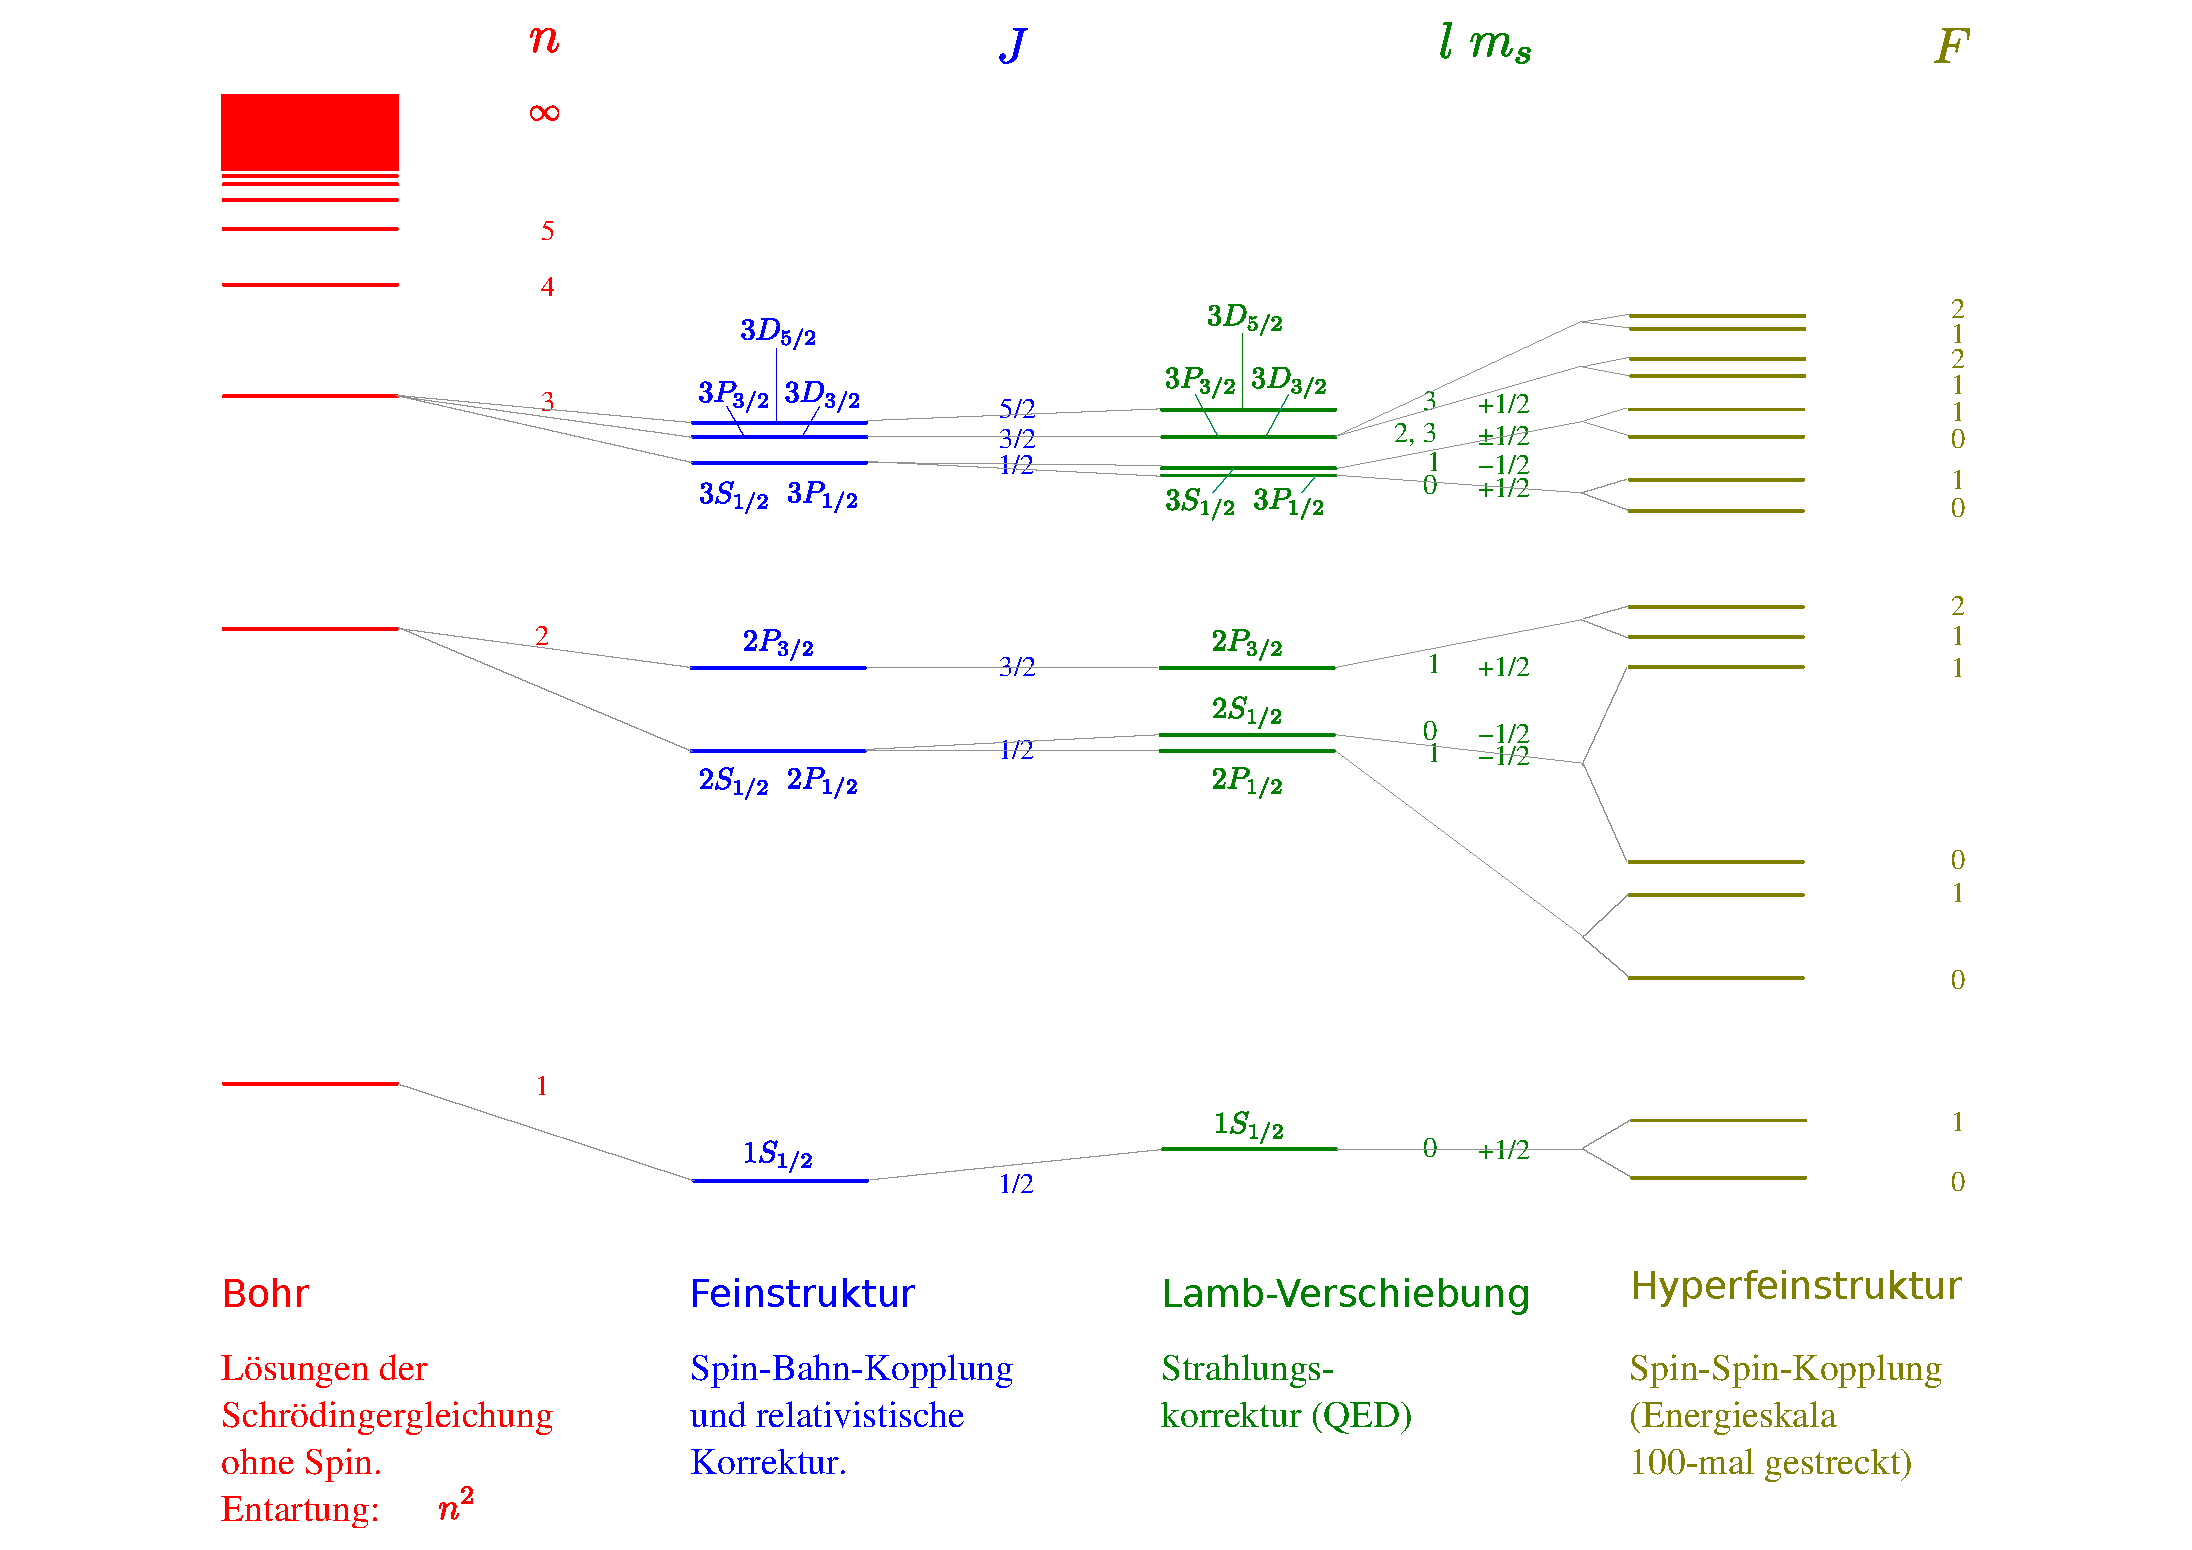
\includegraphics[width=\hsize]{images/WasserstoffAufspaltung.pdf}
\caption{Aufspaltung der Energieniveaus des Wasserstoffatoms (links)
durch die verschiedenen Effekte.
\label{skript:wasserstoffaufspaltung}}
\end{figure}
Die St"orungstheorie kann so die tats"achlich beobachteten Spektren
mindestens qualitativ erkl"aren.
In Abbildung~\ref{skript:wasserstoffaufspaltung} sind links die Energieniveaus
des Wasserstoffatoms dargestellt, wie wir sie im Kapitel~\ref{chapter:wasserstoff}
berechnet haben.
Alle Niveaus sind hochgradig entartet.
Wir werden sp"ater sehen, dass sich die entarteten Zust"ande des
Wasserstoffatoms mit Hilfe des Drehimpuls unterscheiden lassen.
Der Drehimpuls "aussert sich in magnetischen Eigenschaften,
"aussere Magnetfelder oder das vom Spin herr"uhrende magnetische Dipolmoment
der Elektronen spaltet daher die Energieniveaus auf.
Der Grundzustand hat keinen Drehimpuls, er wird daher nur wenig
aufgespalten.

%
% XXX Zeitabhaengige Stoerungstheorie
%
%\section{Zeitabh"angige St"orungstheorie}

\section*{"Ubungsaufgaben}
\rhead{"Ubungsaufgaben}
\begin{uebungsaufgaben}
\item
\input uebungsaufgaben/10001.tex
\item
\input uebungsaufgaben/10002.tex
\end{uebungsaufgaben}
